\documentclass{article}

\usepackage[utf8]{inputenc}
\usepackage{outlines}
\usepackage{amsmath}
\usepackage{cleveref}
\usepackage{graphicx}

\graphicspath{./docs/Figures/}

\usepackage[margin=1in]{geometry}
\parskip 1.5ex % paragraph spacing


\title{Temp RM}
\author{Tom}
\date{January 2021}

\begin{document}

\maketitle

\section{Introduction}
\begin{outline}
    \1 Temperature is a universal force in ecological systems
        \2 Temperature has wide ranging effects
        \2 Works across multiple scales of organisation
    \1 of particular interest is how temperature affects ecosystem dynamics 
        \2 discuss studies looking at how temperature affects stability and other measures
    \1 One potentially overlooked aspect is feasibility 
        \2 define feasibility
        \2 discuss how it is oft negliected aspect of ecosystem dynamics
        \2 is important as:
            \3 a prerequisite for other aspects of dynamics (stability, reactivity ect) 
            \3 An way to explore species sorting and its consequences for measures such as species diverstiy ect...  
\end{outline}

Temperature has long been recognised as fundamental driver of many ecological processes, affecting processes occurring at multiple levels. There is a wealth of evidence documenting these effects anywhere from the effects of temperature on individual physiology,  population growth up to community and ecosystems dynamics. These 

\section{Methods}

\subsection{Theory}
\subsubsection{Model}
In order to explore feasibility and its temperature dependence we use the generalised Lottka-Volterra model (GLV) (REF). This framework is commonly used to explore ecosystem dynamic properties and is regularly applied to study complex, multi-species communities (REF). The GLV describes the dynamics of an $N$ species system where the growth of species $i$ is given by:

\begin{equation} \label{EQ:GLV}
  \frac{1}{x_i} \frac{dx_i}{dt} = r_i - a_{ii} x_i - \sum^N_{i \neq j} a_{ij} x_j, 
\end{equation}

where $x_i$ is the biomass of the $i$th species, $r_i$ is it's intrinsic growth rate, determining the rate at which new biomass is produced ($\text{mass} \cdot \text{time}^{-1} \cdot \text{mass}^{-1} $) and $a_{ij}$ describes the effect of interactions with species $j$ on $i$ (with the $a_{ii}$ term representing intraspecific interactions; $\text{mass}^{-1} \cdot \text{time}^{-1}$). As we want to determine the feasibility of this system (i.e. whether the system will support non-zero biomasses for all species at equilibrium) we need to derive an expression for the equilibrium biomasses. Though it is not possible to derive an exact analytical solution for the GLV as described in \cref{EQ:GLV}, we can use a mean-field approximation, developed by (REF) to get estimate of equilibrium biomass (Supplementary Material). This approximation works by considering interaction term from \cref{EQ:GLV}, which we can rewrite as:

\begin{equation} \label{EQ:mean_int} 
    \sum^N_{i \neq j} a_{ij} x_j = (N-1) \bar{a x} = (N-1) \bar{a} \bar{x} + (N-1) \text{cov}(a,c),
\end{equation}

where the bar notation, $\bar{\cdot}$, represents the average of that quantity over all $N$ species in the system. \Cref{EQ:mean_int} partitions the effects of interactions on the $i$th species into the average effect across the system, $\bar{a} \bar{x}$, and the covariance between heterospecific's biomass and the strength of interactions, $\text{cov}(a,x)$. The mean-field approximation makes two assumptions here: 1) that the covariance term is negligible, which is equivalent to saying that any individual interaction between the focal species and another species population has little effect on that heterospecific's biomass and 2) as long as the system we consider is large, the difference between the average biomass across the system and that of heterospecifics is small (on the order of $N^{-1}$) and can thus be ignored. We also make the further assumption for simplicity that intraspecific interactions are constant across species, setting $a_{ii} = 1$, the implications of are discussed further in (supplementary material?). Combining \cref{EQ:GLV,EQ:mean_int}  we can then express population dynamics in terms the average interaction strength, giving the full mean-field model:

\begin{equation} \label{EQ:MF}
    \frac{1}{x_i} \frac{dx_i}{dt} \approx r_i - x_i - \bar{a}\bar{x}.
\end{equation}

By setting \cref{EQ:MF} equal to $0$ and solving for $x_i$ we then obtain an expression for equilibrium biomass (see Supplementary):

\begin{equation}\label{EQ:MF_eqi}
  x^*_i = K_i -  \bar{K}  \frac{ (N-1)\bar{a}}{1 + (N-1)\bar{a}}, 
\end{equation}

where $K_i = \frac{r_i}{a_{ii}}$ is the carrying capacity, the biomass a population would reach if grown in isolation (obtained by solving \cref{EQ:MF} with $\bar{a} = 0$). \cref{EQ:MF_eqi} provides an intuitive expression for the equilibrium biomasses; a species is expected to reach the biomass that it would in isolation (first term of the RHS, $K_i$) minus the effects of any interspecific interactions (second term on RHS). The strength of these interspecific effects is determined by the average biomass heterospecifics would reach ($\bar{K}$) and a saturating function of interaction strength experienced by the focal species $(N-1)\bar{a}$. If interactions are overall competitive (i.e. $ \bar{a} > 0$) then we see a reduction in equilibrium biomass relative to the individual carrying capacities whereas if they are facilitate ($ \bar{a} < 0$) we see an increase.  

\subsection{Feasibilty}
We use \Cref{EQ:MF_eqi} to derive an expression for the feasibility of a system in terms of the population demographic parameters (i.e. the $r_i$'s and $a_{ij}$'s). We start by recalling that a system is feasible if all species have non-zero equilibrium biomass (i.e. $x_i^* > 0 $), allowing us write a condition for feasibility of a single population. This condition must hold across all populations in order for feasibility of the whole system to be ensured:

\begin{align} \label{EQ:Feas_sp}
  \kappa_i > \frac{(N-1)\bar{a}}{1 + (N-1)\bar{a}} \quad \text{for all} \quad i = 1 \ldots N,
\end{align}

where $\kappa_i = \frac{K_i}{\bar{K}}$ is the mean-normalised carrying capacity. \Cref{EQ:Feas_sp} shows how a system is feasible as long as the the negative effects of interspecific interactions on the each population (RHS) do not outweigh the effects of intraspecific interactions (LHS). We tested the predictions 

\begin{figure}
    \centering
    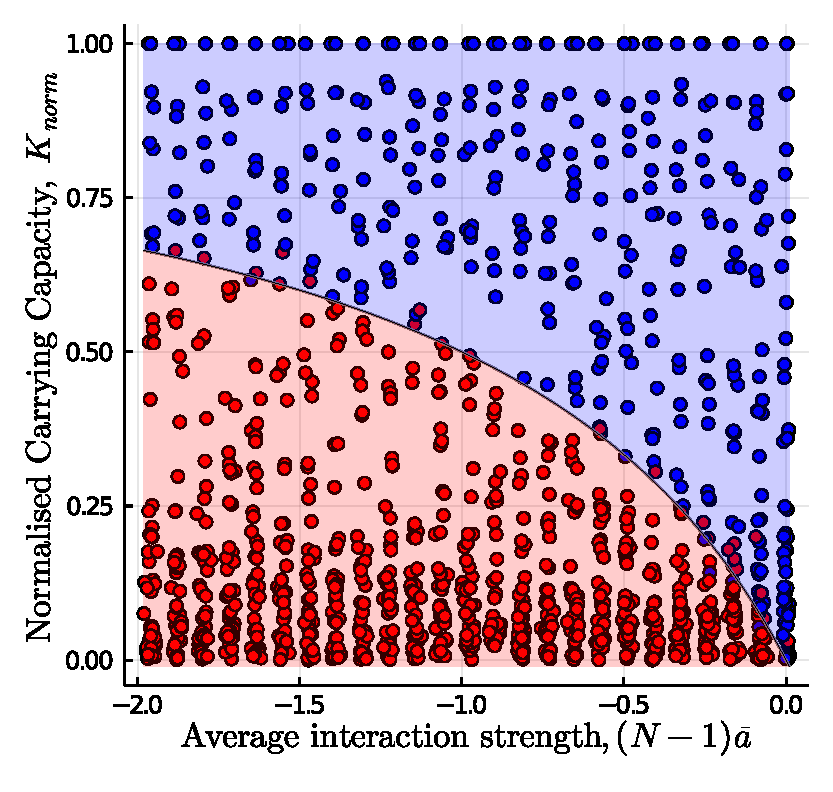
\includegraphics[width = 0.95\textwidth]{docs/Figures/Fig_1.pdf}
    \caption{Caption}
    \label{fig:Feasability_Bound}
\end{figure}

\subsection{Temperature}
In order to relate the condition for feasibility in \cref{MF_feas} to temperature we consider how temperature affects the underlying parameters affecting population dynamics, the growth rates and and  interactions across the ecosystem. To do so we use the Boltzmann-arrhenius equation which describrs the rate of some process $B(T)$ as an exponential-like function of temperature 

There is a wealth of evidence showing that these traits vary with temperature, with variation in the thermal 

As these processes are ultimately dependent on the metabolic rate of individuals (i.e. their ability to transform and utilise resources and energy from the environment) it follows that any any effect of temperatute on metabolism will affect these processes too. The effects of temperature on metabolism can be 

\end{document}
